\chapter{Pufferfish: A space and time-efficient compacted de Bruijn graph index\protect\footnote{A joint work with Hirak Sarkar.}}
\label{sec:pufferfish}


%\section{Abstract}
%  We present a novel data structure for representing the compacted \dbg for use
%  as a pattern matching index. As the popularity of the \dbg as an index has
%  increased over the past few years, so have the number of proposed
%  representations of this structure. Existing structures typically fall into two
%  categories; those that are hash-based and provide very fast access to the
%  underlying k-mer information and those that are space-frugal and provide
%  asymptotically efficient but practically slower pattern search.
%
%  Our representation achieves a compromise between these two extremes. By
%  building upon a minimum perfect hash function, we provide practically fast
%  k-mer lookup, but by carefully organizing our data structure and making use of
%  succinct representations where applicable, we greatly reduce the space
%  compared to traditional hashing-based implementations. Further, we provide the
%  ability to sample positional information, providing the user with the ability
%  to trade off space for speed in a fine-grained manner.
%
%  We believe this representation strikes a desirable balance between speed and
%  space usage, and it will allow for fast search and read mapping on large
%  reference sequences.
%
%
%% \begin{keywords}
%% de Bruijn Graph, compacted de Bruijn Graph, colored de Bruijn graph, kmer, index, read mapping
%% \end{keywords}
%

%%%%%%%%%%%%%%%%%%%%%%%%%%%%%%%%%%%%%%%%%%%%%%%%%%%%%%%%%%%%%%%%%%%%%%%%%%%%%%%%
\section{Introduction}\label{sec:intro}
%%%%%%%%%%%%%%%%%%%%%%%%%%%%%%%%%%%%%%%%%%%%%%%%%%%%%%%%%%%%%%%%%%%%%%%%%%%%%%%

The \dbg is a widely-adopted stucture for genome and transcriptome
assembly~\cite{grabherr2011full,pevzner2001eulerian,haas2013novo}. However, the
compacted variant of the \dbg recenly gained increasing attention both as an indexing
data structure---for use in read alignment~\cite{liu2016debga} and
pseudoalignment~\cite{Bray2016Kallisto}---as well as a structure for analysis of
variation (among multiple genomes)~\cite{minkin2016twopaco}.


%OTHER PAPERS FOR WHICH WE NEED TO WORK IN CITATIONS
%\begin{itemize}
%\item HiSAT2~\cite{kim2015hisat}
%\item BGREAT~\cite{limasset2016read}
%\item GenomeMapper~\cite{schneeberger2009simultaneous}
%\item Gramtools~\cite{maciuca2016natural}
%\end{itemize}


As an indexing data structure, the compacted \dbg is particularly attractive for
dealing with repetitive sequences, since exactly repeated sequences of length at
least $k$ are represented only once in the set of contigs. As has been
demonstrated by~\cite{liu2016debga}, this considerably speeds up alignment
to repeat-heavy genomes (e.g., the human genome) as well as collections of
related genomes. Further, it has also been demonstrated by Bray et al.~\cite{Bray2016Kallisto}, 
that if full alignment information is not needed, a
properly-indexed compacted \dbg also supports very efficient queries to
determine the reference sequences compatible with sequenced reads (i.e.,
pseudoalignment).

However, the speed of existing compacted \dbg indices comes at a considerable
cost in index size and memory usage. Specifically, the need to build a hash
table over the k-mers appearing in the \dbg contigs requires a large amount of
memory, even for genomes of typical size. Typically, these hash functions map
each k-mer (requiring at least 8 bytes) to the contig in which it occurs
(typically 4 or 8 bytes) and the offset where the k-mer appears in this contig
(again, typically 4 or 8 bytes). A number of other data structures are also
required, but this hash table most of the time dominates the overall index size. For
example, an index of the human genome constructed in such a manner (i.e., by
deBGA or kallisto) requires $70$---$100$GB of RAM. This already exceeds the
memory requirements of moderate servers (e.g., those with 64G of RAM), and these
requirements quickly become untenable with larger genomes or collections of
genomes.

\begin{figure}
  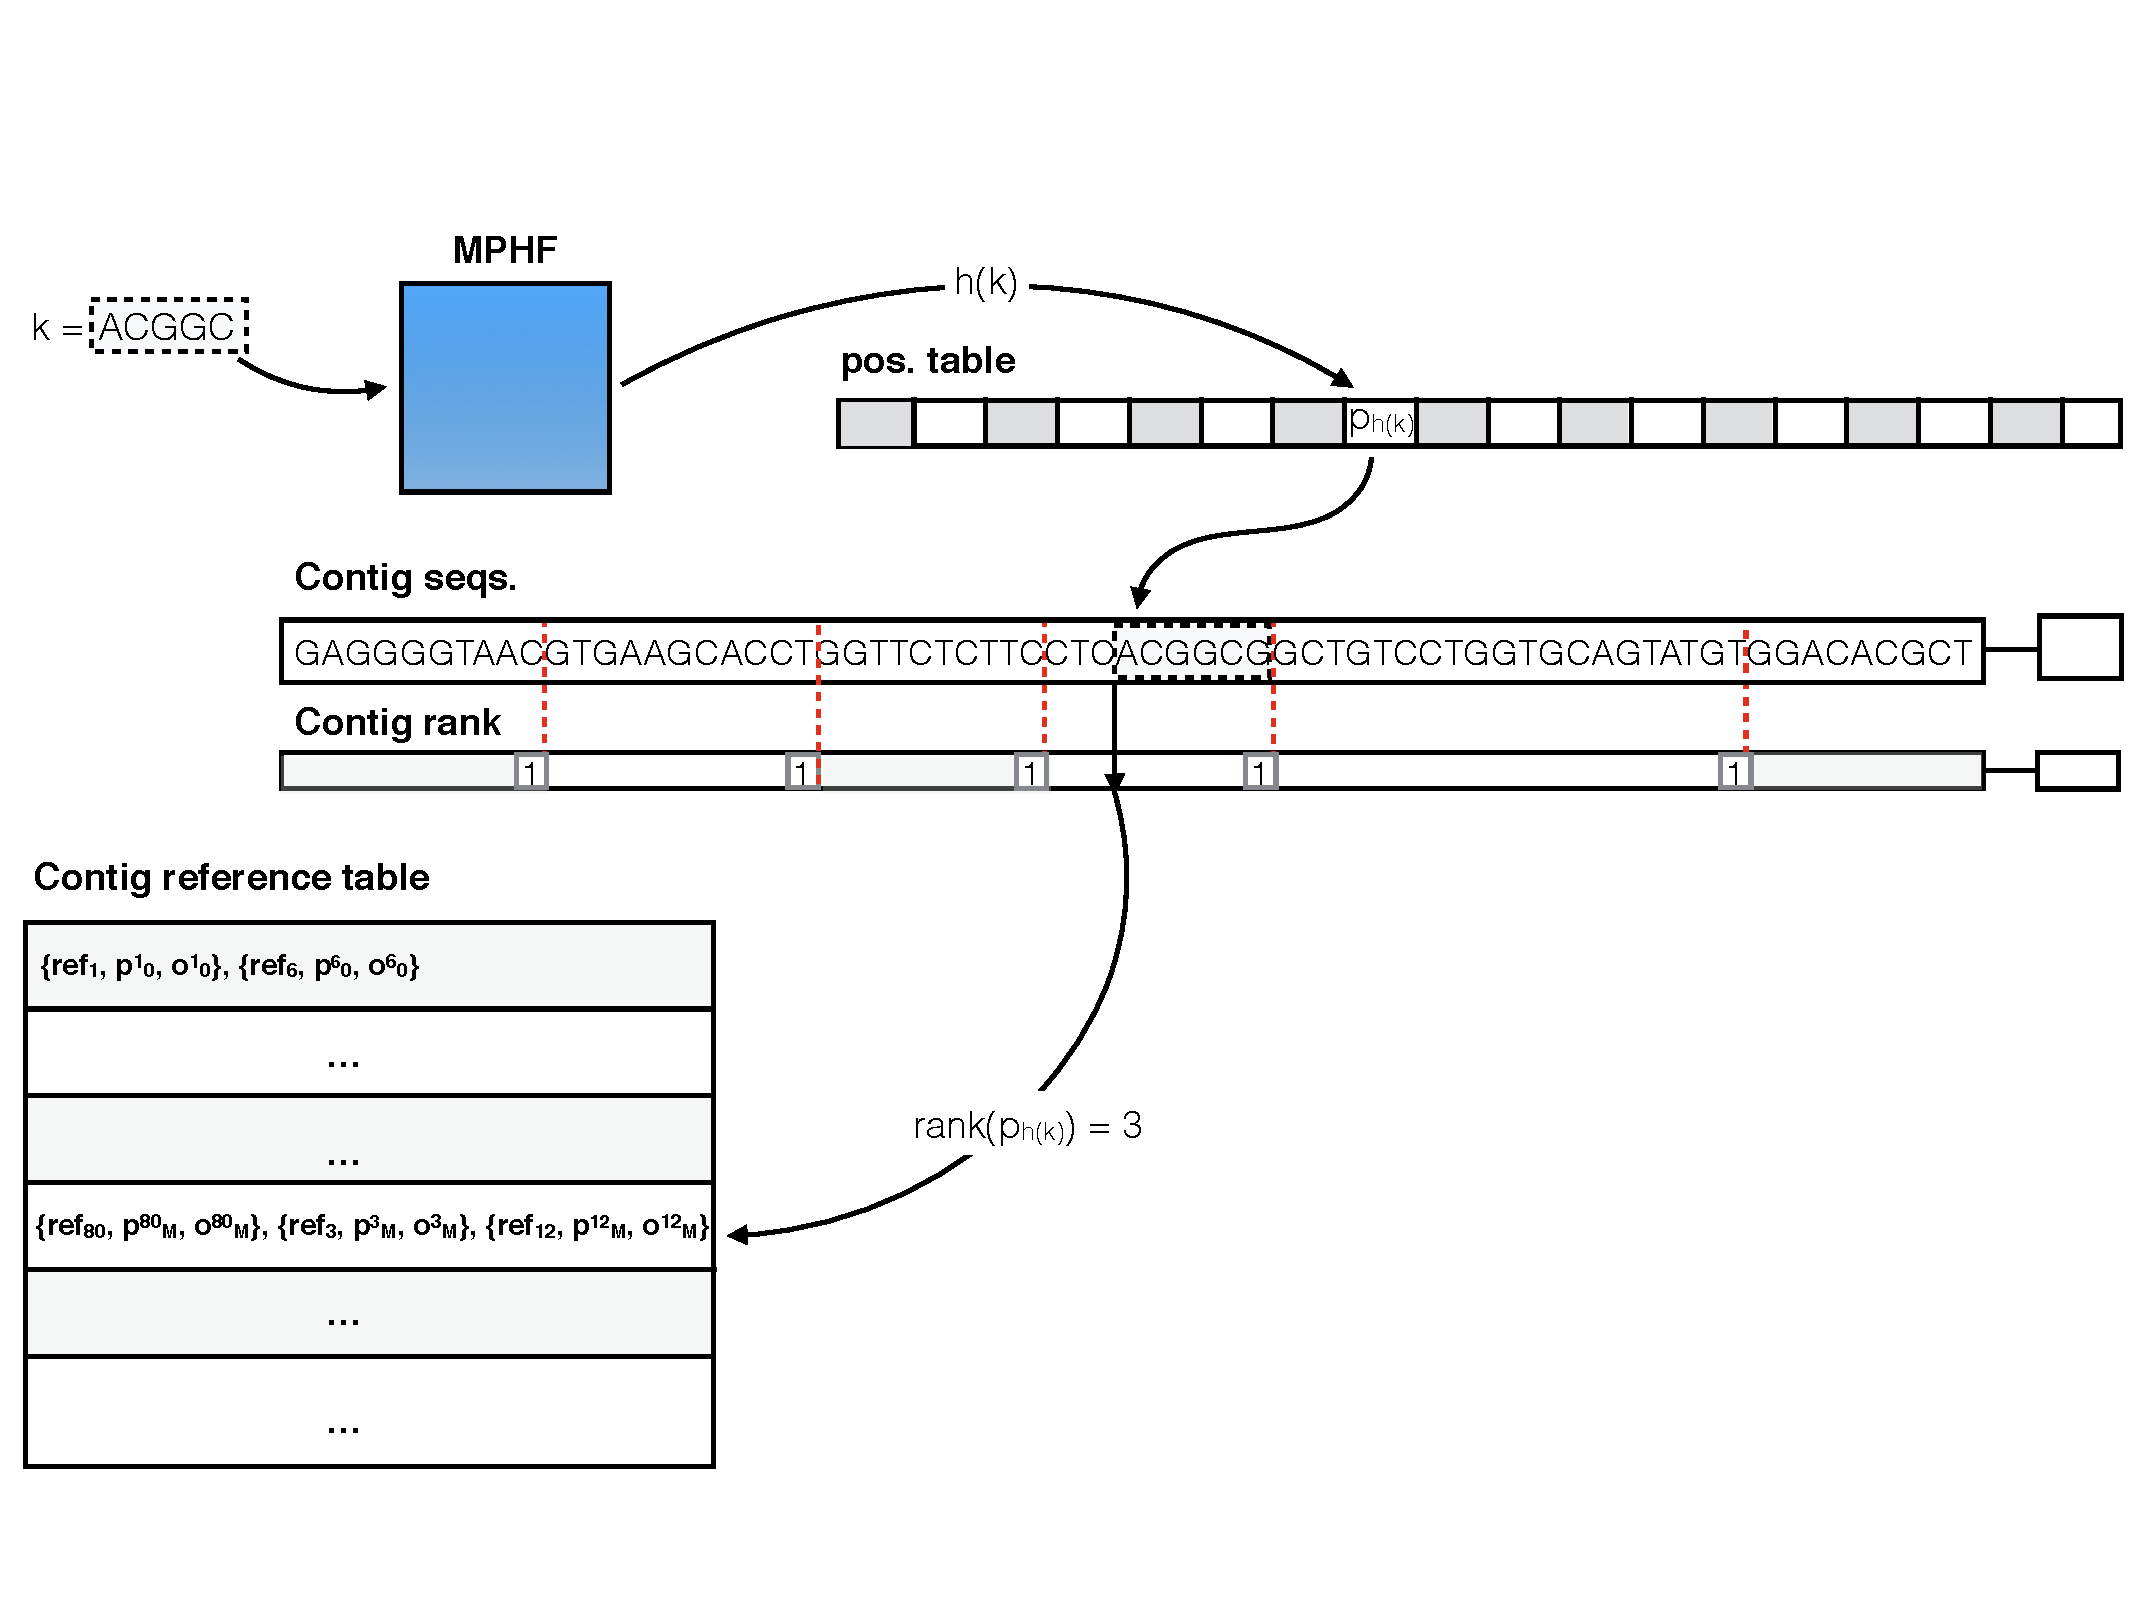
\includegraphics[width=\textwidth]{figs/index_fig}
\caption{An illustration of searching for a particular \kmer in the \emph{dense}
  \pufferfish index. The minimum perfect hash yields the index, $P_{h(x)}$ in the
  \emph{pos} vector where the \kmer appears in the contig array. The \kmer is
  validated against the sequence recorded at this position (and, in this case,
  it matches). A rank operation on $p_{h(x)}$ is performed in the boundary
  vector, which yields the corresponding contig-level information in the contig
  table. If desired, the relative position of the \kmer within the contig can be
  retrieved with an extra select and rank operation.}
\label{fig:dense_index}
\end{figure}


\section{Methods}\label{sec:methods}

We introduce a new data structure, implemented in the software \pufferfish, for
indexing the \ccdbg (and colored variants of it). While we are conscious of
memory usage, we don't aim to build the smallest possible index. Rather, we care
about making the \ccdbg index practical for genomic and metagenomic data while
maintaining very fast query speeds over the index. Here, we introduce both a
\emph{dense} and \emph{sparse} variant of the \pufferfish index, where, as with the
FM-index~\cite{Ferragina2001Experimental}, the sparsity factor can be tuned to
trade off search speed for index size. The sparse index tuned to take maximum space,
is at the same level as dense index regarding space and \kmer query time.

\paragraph*{Pre-processing} We assume as input to \pufferfish, the \ccdbg on the reference
or set of references to be indexed. The \pufferfish software itself accepts as input
a graphical fragment assembly (GFA) format file that describes the \ccdbg.
Specifically, this file encodes the contigs (i.e., non-branching paths) of the
\ccdbg as ``segments'' and the mapping between these contigs and the original
reference sequences as ``paths''. Each path is spelled out with an ordered set of contig IDs and the orientation they are mapped by, so that each contig has an overlap of k-1 with its following contig in the path (either in forward or reverse-complement).
The GFA is an evolving standard that is meant
to be a common format used by tools dealing with graphical representations of
genomes or collections of genomes. We note that there are a number of software
tools for building the \ccdbg directly (i.e., without first building the
un-compacted \dbg). We adopt \twopaco~\cite{minkin2016twopaco}, which employs a
time and memory-efficient, parallel algorithm for directly constructing the
\ccdbg, which can then easily be converted into GFA format. We note that, due to
a technical detail in the way \twopaco constructs the \ccdbg and the GFA file,
this output cannot be used directly, so \pufferfish includes a GFA-to-GFA converter
that prepares the \twopaco-generated GFA file for indexing by
\pufferfish\footnote{Specifically, the \twopaco \ccdbg has two main differences with
  the format that is expected by \pufferfish. First, it is not the case that \kmers
  and their reverse complements will appear only once in the \twopaco \ccdbg.
  Second, the GFA generated by \twopaco assumes that \emph{edges} of size at
  least $k+1$ will act as GFA segments, implying that they will overlap by $k$
  nucleotides. However, we require that segments be of at least size $k$ and
  overlap by exactly $k-1$ nucleotides.}.

\subsection*{The dense \pufferfish index}

Here we describe the basic (i.e., dense) \pufferfish index. The index consists of 6
components, each of which is described below:

\begin{enumerate}

\item The contig sequence array (\cseq) consists of the (2-bit encoded) sequence of all
  contigs of the \ccdbg packed together into a single array. Typically, the size
  of this structure is close to (or smaller than) the size of the 2-bit encoded
  reference sequence, since redundant sequences are represented only once in
  this structure. We note that the contig array contains the sequence of every
  valid \kmer, as well as that of potentially invalid \kmers (those which span
  contig boundaries in the packed array as the contig sequences in the array follow each other without any delimiters or gaps.).
  Therefore, using the next data structure we will set the boundaries of contigs in the array in a way that makes retrieving the borders, knowing position of a contig in the contig array and length of the contig fast in the query process. 
  We denote by $L_s$ the total length (in
  nucleotides) of the contig array.

\item The boundary vector (\bv) is a sparse bit-vector with a length of $L_s$
  bits. The bits of this vector are in one-to-one correspondence with the
  nucleotides of the contig array, and the boundary vector contains a one at
  each nucleotide corresponding to the end of a contig in the contig array, and
  a zero everywhere else. We can retrieve rank of each contig in \cseq using the
  \rank~operation on \bv. $\rank(\bv[i])$ returns number of 1s in \bv before the current index, $i$, or in other words the rank of the current contig. This can be used to get reference information for the current contig from \ctab, the data structure explained in item \ref{items:dense5}.

\item The minimum perfect hash function ($h\left(\right)$) maps every
  \emph{valid} \kmer in the contig array (i.e., all \kmers not spanning contig
  boundaries) to a unique number in $\left[0,N\right)$, where $N$ is the number
    of distinct valid \kmers in \cseq. We make use of the highly-scalable MPHF
    construction algorithm of~\cite{limasset2017fast}.

\item The position vector (\emph{pos}) stores, for each valid \kmer $x$, the
  position where this \kmer occurs in \cseq. Specifically, for \kmer $x$,
  \emph{pos}$\left[h\left(x\right)\right]$ contains the starting position of $x$ in \cseq 
  such that $\cseq\left[h\left(x\right),h\left(x\right) + k\right] = x$.

\item The conitg table \ctab stores, for each contig appearing in \cseq, the reference
  sequences (including reference ID, offset and orientation) where this contig appears in the
  reference. This is similar to a ``posting list'' in traditional inverted
  indices, where all occurrences of the item (in this case, an entire \ccdbg
  contig) are listed. The order of the contigs in the contig table is the same
  as their order in \cseq, allowing the information for a contig to be accessed
  via a simple rank operation on \bv.

\label{items:dense5}

\item \emph{Optionally}, an equivalence class table that records, for each
  contig, the set of reference sequences where this contig appears.
  Pre-computation and storage of these equivalence classes can speed up fast
  mapping approaches (e.g., pseudoalignment).

\end{enumerate}

These structures allow us to index every \kmer in the \ccdbg efficiently, and to
recall, on demand, all of the reference loci where this \kmer occurs. We note
here that the \kmers of the \ccdbg constitute only a subset of the \kmers in
\cseq. We refer to all \kmers in \cseq that do not span the boundary between two
contigs as \emph{valid} \kmers; these are in one-to-one correspondence with the
\kmers of the \ccdbg.

\subsubsection*{\kmer query in the dense \pufferfish index}
By using a MPHF $h$ to index the \emph{valid} \kmers, we avoid the typically
large memory burden associated with standard hashing approaches. Instead, the
identity of the hashed keys is encoded implicitly in \cseq. Given a \kmer $x$, we
can check for its existence and location in the following way. We first compute
$i = h(x)$, the index assigned to \kmer $x$ by $h$. If $i > N$, then we
immediately know that $x$ is not a valid \kmer. Otherwise, we retrieve the
position $p_{i}$ stored in $\texttt{pos}[i]$. Finally, we check if the encoded
string $\cseq[i:i+k]$ is identical to $x$. If so, we have found the
contig location of this \kmer, otherwise, $x$ is not a valid \kmer. 

Given $p_{i}$, we can retrieve the reference positions by computing $r_{p_i} =
\rank(\bv[p_{i}])$, which provides an index into \ctab that is
associated with the appropriate contig. This provides all of the reference
sequences, offsets and orientations where this contig appears. We compute the
offset of \kmer $x$ in the contig as $o_{i} = p_{i} - \select(r_{p_i})$,
in which \select returns the start position of the contig in \ctab.
This allows us to easily project this \kmer's position onto each reference
sequence where it appears. We note that querying a \kmer in the \pufferfish index is
an asymptotically constant-time operation, and that the reference loci for a
\kmer $x$ can be retrieve in $O(\texttt{occ}(x))$ time, where $\texttt{occ}(x)$
is the number of occurrences of $x$ in the reference.

\subsection*{The sparse \pufferfish index}

The \pufferfish index, as described above, is relatively memory-efficient. Yet, what
is typically the biggest component, the \texttt{pos} vector, can still grow rather
large. This is because it occupies $\lg(L_s)$ bits for each of the $N$ valid
\kmers in \cseq. However, at the cost of a slight increase in the practical
(though not asymptotic) complexity of lookup, the size of this structure can be
reduced considerably. To see how, we first make the following observation:

\begin{observation}
  In the \ccdbg (and hence, in \cseq), each valid \kmer occurs exactly once (\kmers occuring between contig boundaries are not considered).
\end{observation}

Hence, any valid \kmer in the \ccdbg is either a complex \kmer (i.e., it has an
in or out degree greater than 1), is a terminal \kmer (i.e., it appears at the
beginning or end of some input reference sequence), or it has a unique
predecessor and successor in the orientation defined by the contig.

We can exploit this observation in \pufferfish to allow \emph{sampling} of the \kmer
positions. That is, rather than storing the position of each \kmer in the contig
array, we store the position only for some subset of \kmers, where the rate of
sampling is defined by a user-defined parameter $s$. For those \kmers that are
not sampled, we store, instead, four pieces of information; the extension that
must be applied to move toward the closest \kmer at a sampled position, whether
or not the corresponding \kmer in \cseq is canonical, whether the extension
to reach the nearest sampled position should be applied by moving to the left or
the right, and a bit vector with the same size as \cseq
that is set to $1$ for any \kmer in \cseq that we've stored its position and $0$
for those that are not sampled.
This idea of sampling the positions for the \kmers is similar to the
idea of sampling the suffix array positions that is employed in the
FM-index~\cite{Ferragina2001Experimental}. This allows us to trade off query
time for index space, to allow the \pufferfish index to scale to large genomes or
collections of genomes. 


\subsubsection*{\kmer query in the sparse \pufferfish index}  \kmer query in the sparse \pufferfish index
is the same as that in the dense index, except for the first step ---
determining the position of the \kmer $x$ in \cseq. When we query the MPHF with
$x$ to obtain $i = h(x)$, there are three possible results. 
\begin{enumerate}
\item In the first case,
we could have that $i \geq N$, implying, just as in the dense case, that $x$ is
not a valid \kmer. 
\item Second, we could have that $\texttt{sampled}[i] = 1$,
implying that we have explicitly stored the position for the $i$-th \kmer, in
which case we can retrieve that position as $p_{i} = \texttt{pos}[\texttt{rank}(\texttt{sampled}[i])]$ and
proceed as before in the dense case to validate $x$ and retrieve its reference positions.
\item The third case is that $i < N$ and $\texttt{sampled}[i] = 0$. In this case, we do not know
the position where $x$ would occur in \cseq, and we must find the closest sampled position.
This is done with algorithm \ref{alg:nextSample}
\end{enumerate}

\begin{algorithm}
\caption{Find Next Sample}\label{alg:nextSample}
\begin{algorithmic}[1]
\Procedure{FindNextSample}{}
\State $\textit{e} \gets \textit{extension} \text{ size}$
\State $X \gets \textit{\kmer}$
\State $EV \gets \text{extension vector}$

\State $i \gets \textit{MPHF(\kmer)}$
\State $X_{rc} \gets \textit{reverseComplement}(X)$
%\BState \emph{loop}:
\While{\textbf{not} $isSampled[i]$} 

%\If {$isSampled[i]$}
%\State \textbf{goto} \emph{end}.
%\EndIf
\State $extIdx \gets i-rank(isSampled[i])$
\If {$isCanonical[i]$ \textbf{and} $isDirectionRight[i]$}
\State $X \gets X[e:] + EV[extIdx]$.
\EndIf
\If {\textbf{not} $isCanonical[i]$ \textbf{and} $isDirectionRight[i]$}
\State $X \gets X_{rc}[e:] + EV[extIdx]$.
\EndIf
\If {$isCanonical[i]$ \textbf{and} \textbf{not} $isDirectionRight[i]$}
\State $X \gets EV[extIdx] + X[:-e]$.
\EndIf
\If {\textbf{not} $isCanonical[i]$ \textbf{and} \textbf{not} $isDirectionRight[i]$}
\State $X \gets EV[extIdx] + X_{rc}[:-e]$.
\EndIf
\State $i \gets \textit{MPHF(\kmer)}$
\State $X_{rc} \gets \textit{reverseComplement}(X)$
\EndWhile
%\BState \emph{end}:
\Return $X$
\EndProcedure
\end{algorithmic}
\end{algorithm}


Intuitively, algorithm \ref{alg:nextSample} appends nucleotides stored in the
\texttt{extension} array to $x$ to generate a new \kmer, $x'$ which either has a
sampled position, or is closer to a sampled position than is $x$. The extension
process is repeated with $x'$, $x''$, etc. until a sampled position is reached.
At that point, one simply traverses back to the position in \cseq implied by the
sampled position and sequence of extension operations, for the original \kmer
$x$. The rest of the search proceeds as for the dense case. The whole process of
\kmer query in sparse index is illustrated in Fig \ref{fig:sparse_query} through an example.

\begin{figure}
  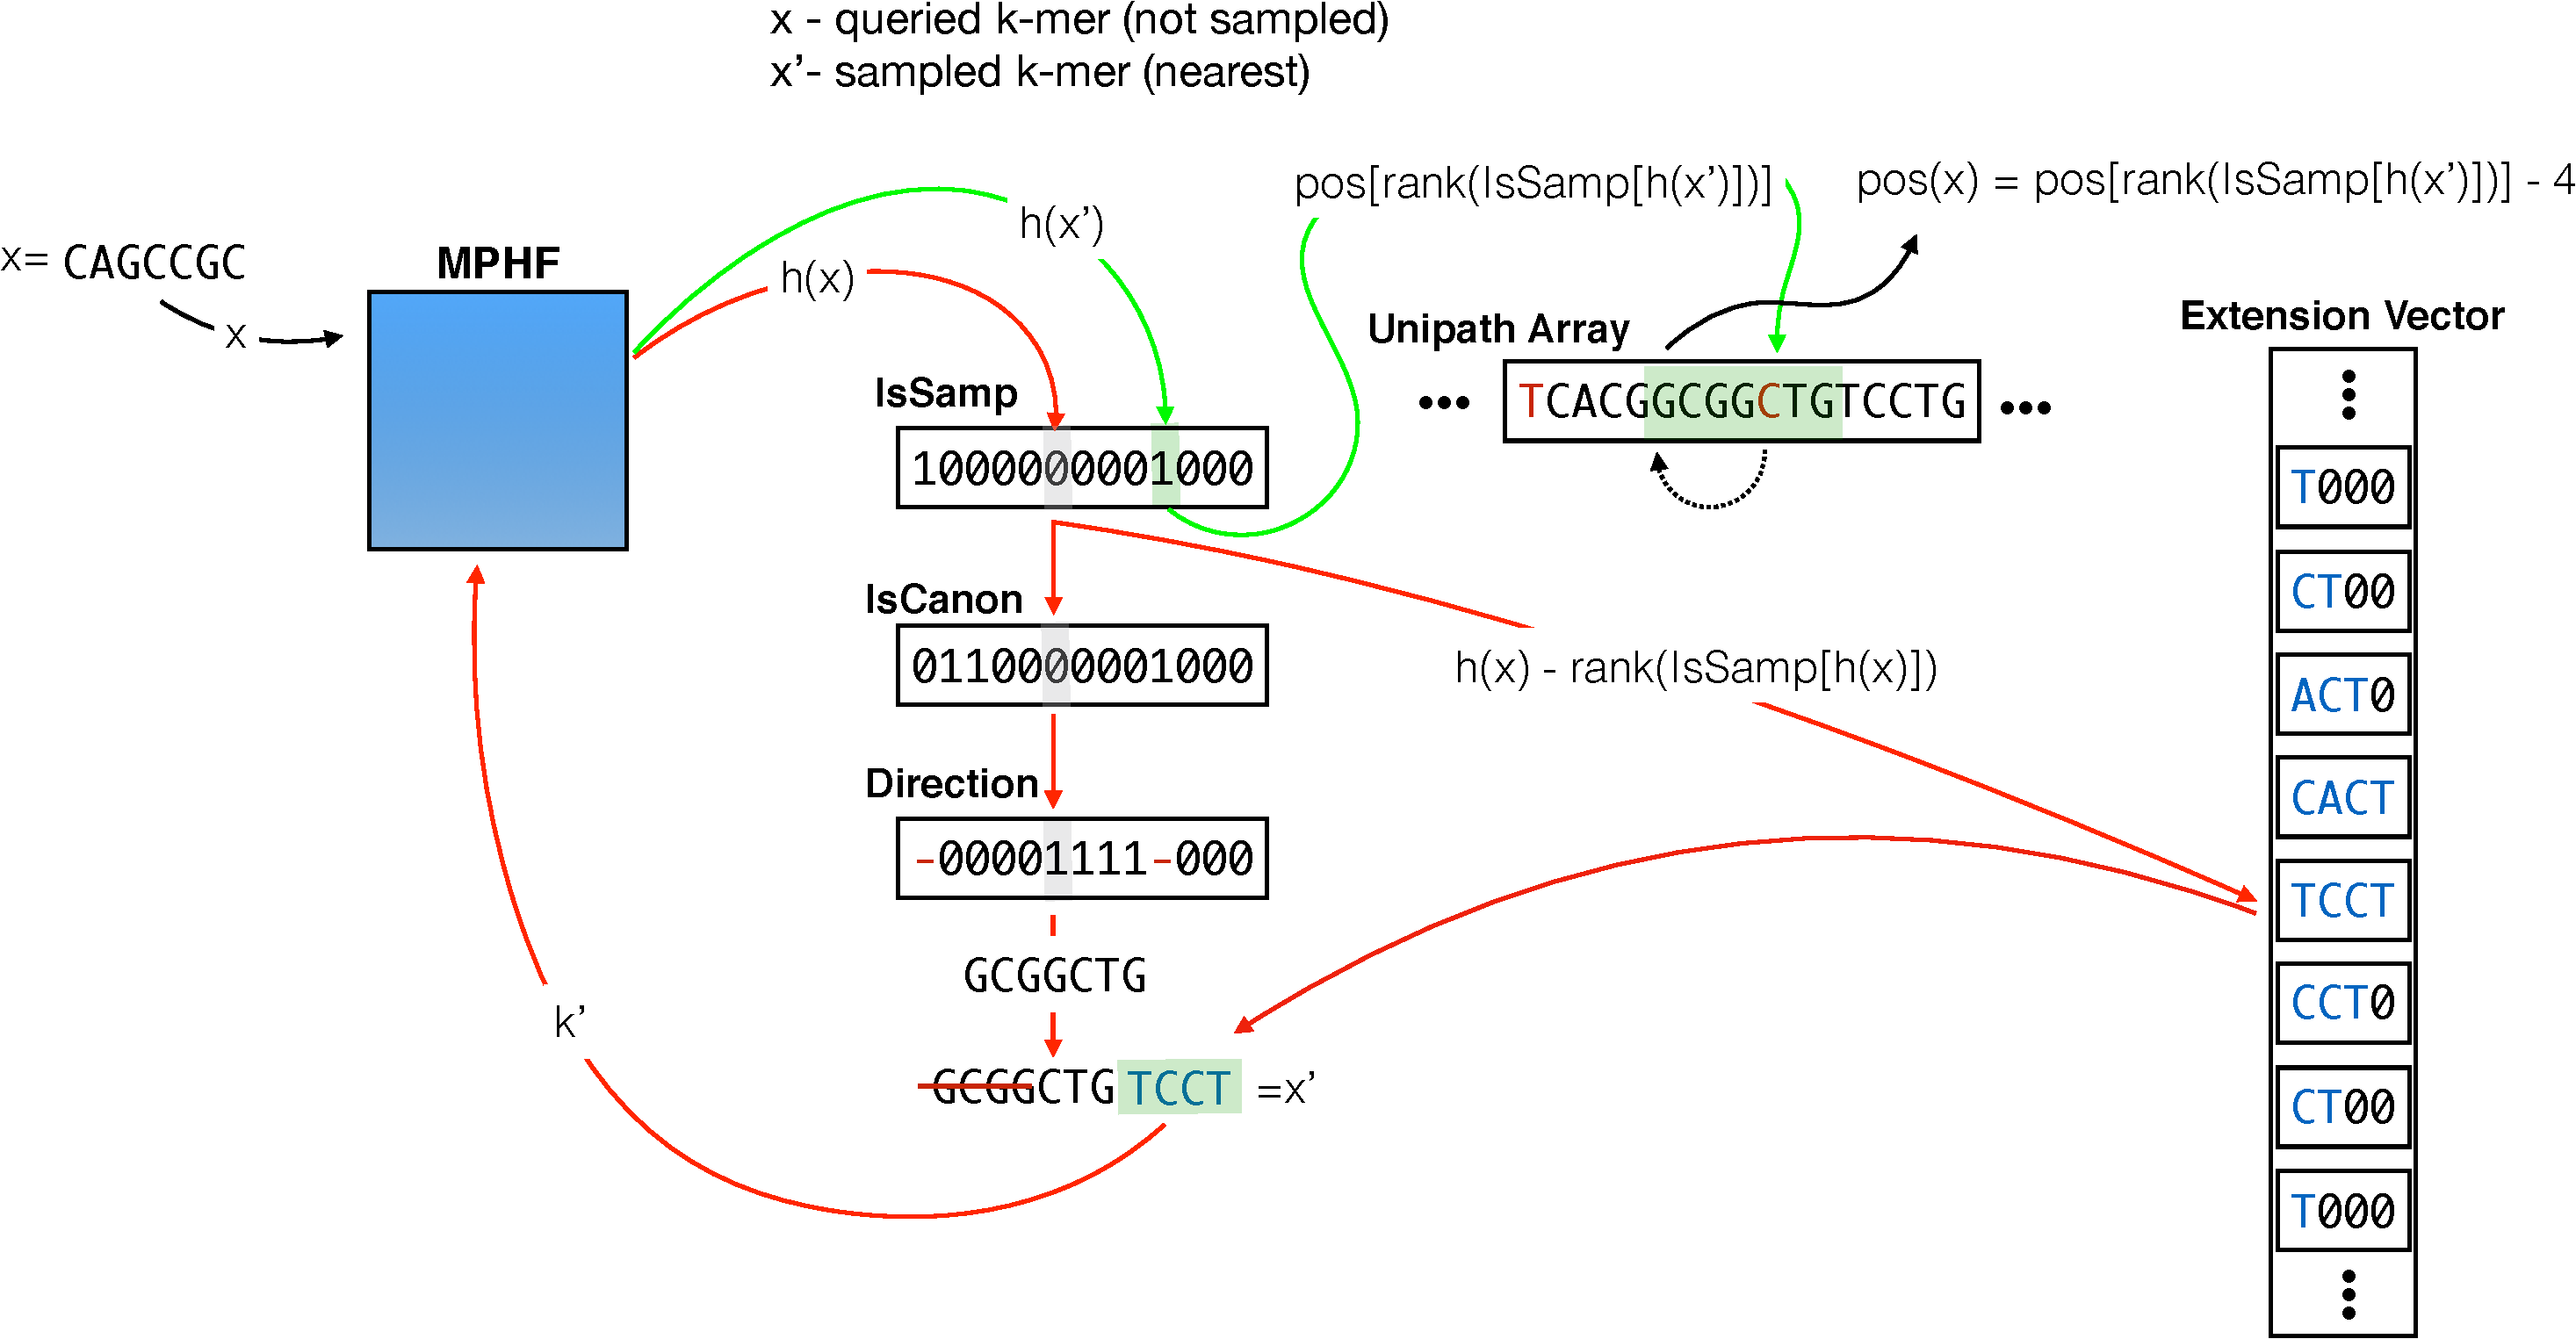
\includegraphics[width=\textwidth]{figs/query_sparse}
\caption{An illustration of searching for a particular \kmer in the \emph{sparse}
  \pufferfish index with sample factor ($s$) of 9 and extension size ($e$) of 4.
  All vectors \emph{isSampled}, \emph{isCanon}, and \emph{ExtRight} have the same
  size which is equal to length of the total number of valid \kmers.
  The minimum perfect hash yields the index, $h(x)$ for $x=CAGCCGC$ in the
  \emph{isSampled} vector where we'll find out that the \kmer is not sampled.
  \emph{isCanon} being $0$ at the same index as $h(x)$ shows that the \kmer
  is not canonical. Since we keep the extensions in canonical format we need to 
  canonicalize the \kmer to $x'=GCGGCTG$ first. Then based on the value of 
  $\text{\emph{ExtRight}}_{h(x)}$, we know that to get to the closest sampled \kmer
  we need to append the extension to the right of the current \kmer.
  The extension is extracted from \emph{QueryExt} vector. Considering the fact
  that we just keep the extensions for \kmers that are not sampled,
  to find the index of the current \kmer's extension we need to
  subtract the index of the \kmer by total number
  of \kmers that have been sampled up to this position which is equal to 
  total number of $1$s in \emph{isSampled} vector before $h(x)$ for which we use the
  \emph{rank} operation. Therefore, the extension index will be $h(x)-rank(isSampled[h(x)])$.
  We create the new \kmer $x'$ by cropping the first four bases off the current \kmer and
  appending the new extension to its right and repeat the same process for the new \kmer.
  This time, the \kmer is sampled and hence, we go directly to the index in the \emph{UnipathArray}
  that the \emph{sampledPos} vector points us to. To check if the original \kmer we searched for
  exists, we need to compare the \kmer starting from $4$ bases before the current position 
  with the canonic of original \kmer $x=CAGCCGC$ since we just appended one extension of size 4
  to the end of this \kmer. Generally speaking, we need to revert all the extension appendings 
  by walking over the \emph{UnipathArray} vector to the left and right with the same steps as
  extension size until we stop at the right position that we expect the \kmer at that position to be the
  same as the one we searched.}
\label{fig:sparse_query}
\end{figure}



By altering the stored extension size $e$ and the maximum sampling rate $s$, one
can limit the maximum number of extension steps (and hence the maximum number of
hash lookups) that must be performed in order to retrieve the potential index of
$x$ in \cseq. A denser sampling and longer extensions require fewer possible
extension steps, while a sparser sampling and shorter extensions require less space
for each non-sampled position. If $e \geq \frac{s}{2}$, one can guarantee that
at most a single extension step needs to be performed for any \kmer query, which
allows \kmer queries to remain, practically very fast while still considerably
reducing the index size for large reference sequences.

Even though the sparse index maintains a number of extra bit vectors not maintained
in the dense index, it is still usually considerably smaller.
Assume a case where the extension length $e$ is half of the sampling factor $s$.
Since we keep the extension required to get to 
the closest position in left or right direction, we would need to keep
$\frac{s}{2}$ bases for a kmer with each base represented in 2 bits, which corresponds to 
$\frac{s}{2}\times 2 = s$ bits per \kmer for the extension vector. Therefore, if we put all the new 
vectors of extension, canonical, direction, and isSampled together it'll be $s+1+1+1=s+3$ bits 
per each non-sampled \kmer compared to $\lg(L_s)$ bits that we had to keep in 
\emph{pos} vector. Therefore, as long as $[s+3< \lg(L_s)]$ we save space by sparse indexing.
In a typical data set such as human genome with $\lg(L_s) \sim= \lg(3B) \geq 30$ bits, by choosing
$s=9$ which means we'll sample each 9th \kmer, we will save $\sim18$ bits per each non-sampled \kmer.
%\todo{put actual numbers}

\section{Results}\label{sec:results}

We explored the memory and time requirements for building a text index using
\pufferfish and two other tools, \bwa and \kallisto. We also benchmark the speed of
\kmer lookup (the fundamental building block of \bwa's alignment and \kallisto's
pesudoalignment) under these different data structures. We performed these
benchmarks on a number of different reference sequences, selected to show how
the different indexes scale as the underlying reference size and complexity
increase. \bwa and \kallisto both have the complete package for
indexing a data set. For \pufferfish however, we first need to build the \ccdbg using the available
tools. We build the \ccdbg and dump it in GFA format using \twopaco. Then, as the output does
not satisfy our definition of a compacted dbg, we need to have another preparation 
step to convert the GFA file. We call this process\emph{pufferization}, and it converts the GFA file to the format accepted by pufferfish
(each \kmer should be appear only once through out all the unitigs and unitigs should have an overlap of $k-1$ bases).
Then we will build both dense and sparse index and benchmark the time and memory for all these steps of the pipeline individually.
Final comparison between the time and memory that pufferfish requires versus the other tools should be the aggregated time and
maximum memory of the whole pufferfish pipeline.
All experiments
were performed on an Intel(R) Xeon(R) CPU (E5-2699 v4 @2.20GHz with 44 cores and
56MB L3 cache) with 512GB RAM and a 4TB TOSHIBA MG03ACA4 ATA HDD running ubuntu
16.10, and were carried out using a single thread except for cdBg building step using TwoPaCo.

%\todo{explain datasets}

\begin{table}
\begin{center}
\begin{tabular} {| l || c c c| c c c|}
\hline
\multirow{2}{*}{Indexing Tools} & \multicolumn{3}{c|}{Memory (MB)} & \multicolumn{3}{c|}{Time (secs)} \\
\cline{2-7}
& \parbox[c]{2.5cm}{Human\vfill Transcriptome} & 
\parbox[c]{1.5cm}{Human\vfill Genome} & 
\parbox[c]{1.5cm}{Bacterial \vfill Genome} & 
\parbox[c]{2.5cm}{Human \vfill Transcriptome} & 
\parbox[c]{1.5cm}{Human \vfill Genome} & 
\parbox[c]{1.5cm}{Bacterial \vfill Genome} \\
\hline
 
\bwa & 292 & 4,443 & 32,213 & 2:56 & 0:58:27 & 13:11:45\\
\hline
\kallisto & 3,552 & 150,657 & NA & 3:05 & 3:27:42 & >2 days\\
\hline
\twopaco & 1,466 & 18,004 & NA & 2:47 & 0:56:12 & >2 days \\
pufferize & 584 & 27,438 & 49,510 & 0:10 & 0:21:53 & 54:11\\
pufferfish dense & 438 &  20,000 & 30,224 & 1:16 & 0:51:20 & 1:27:08 \\
pufferfish sparse & 331 & 17,745 & 29,811 & 1:44 & 1:10:48 & 2:02:34\\
\hline
\end{tabular}
\caption{
  Construction time and memory for \pufferfish, \kallisto, and \bwa for different
  datasets. 
}
\vspace{-2.5em}
\label{tab:construction}
\end{center}
\end{table}

\begin{table}
\begin{center}
\begin{tabular} {| l || c c c| c c c|}
\hline
\multirow{2}{*}{Indexing Tools} & \multicolumn{3}{c|}{Memory (MB)} & \multicolumn{3}{c|}{Time (secs)} \\
\cline{2-7}
& \parbox[c]{2.5cm}{Human\vfill Transcriptome} & 
\parbox[c]{1.5cm}{Human\vfill Genome} & 
\parbox[c]{1.5cm}{Bacterial \vfill Genome} & 
\parbox[c]{2.5cm}{Human \vfill Transcriptome} & 
\parbox[c]{1.5cm}{Human \vfill Genome} & 
\parbox[c]{1.5cm}{Bacterial \vfill Genome} \\
\hline
 
         
  
\bwa & 308 & 4,440 & 33,333 & 1:09:14 & 1:11:29 & 6:41\\
\hline
\kallisto & 3,337 & 110,646 & 120,748 & 6:17 & 24:29 & 20:06\\
\hline
pufferfish dense & 500 & 17,661 & 28,596 & 6:05 & 16:14 & 3:34 \\
pufferfish sparse & 315 & 12,510 & 20,470 & 17:41 & 26:38 & 4:26\\
\hline
\end{tabular}
\caption{
  \kmer lookup time and memory for \pufferfish, \kallisto, and \bwa for different
  datasets. 
}
\vspace{-2.5em}
\label{tab:query}
\end{center}
\end{table}

As expected we see in table \ref{tab:construction} that \pufferfish takes longer to build the index compared to a linear indexing based
tool such as \bwa and stands almost in the same level as \kallisto which is another graph-based indexing tool. 
However, the amount of memory it needs is considerably smaller than \kallisto, so that for a large reference
such as the human genome, it consumes $\sim6$ times less memory. Comparing the \kmer lookup time in table \ref{tab:query}, 
we can see how using a graph-based indexing system can outperform \bwa regarding time and still because of the succinct
data structures used in the index building and the compression algorithms used in that would need almost the same memory as \bwa
which is much less than what \kallisto needs to load all the indexing data structure.
The disk space and memory \pufferfish needs are very similar, unlike \kallisto, where the hash table consumes
much more RAM than what serialized version requires on disk.

\begin{table}
\begin{center}
\begin{tabular} {| l || c c c |}
\hline
\parbox[c]{2cm}{Indexing \vfill Tools} & 
\parbox[c]{2.5cm}{Human\vfill Transcriptome} & 
\parbox[c]{1.5cm}{Human\vfill Genome} & 
\parbox[c]{1.5cm}{Bacterial \vfill Genome}  \\
\hline   
       
\bwa & 347M & 5.12G & 37.8G \\
\hline
\kallisto & 1.7G & 58G & 87G \\
\hline
pufferfish dense & 387M & 16G & 26G \\
pufferfish sparse & 271M & 11G & 18G \\
\hline
\end{tabular}
\caption{
  Disk space each of \pufferfish, \kallisto, and \bwa will take for different
  datasets. 
}
\vspace{-2.5em}
\label{tab:disk-space}
\end{center}
\end{table}
%kallisto construction on GRCh38 (primary)
%%
%rob@newton:~ /usr/bin/time ~/kallistokmerlookup/build/src/kallisto index -k 31 -i GRCh38.primary\_assembly.genome.fixed.kalidx GRCh38.primary\_assembly.genome.fixed.fa
%
%[build] loading fasta file GRCh38.primary\_assembly.genome.fixed.fa
%[build] k-mer length: 31
%[build] counting k-mers ... done.
%[build] building target de Bruijn graph ...  done
%[build] creating equivalence classes ...  done
%[build] target de Bruijn graph has 38967126 contigs and contains 2652229049 k-mers
%
%7911.72user 1873.99system 2:45:24elapsed 98\%CPU (0avgtext+0avgdata 154270332maxresident)k
%0inputs+119758728outputs (0major+3389704442minor)pagefaults 0swaps
%%

We note that on large sequences (e.g., the human genome)
kallisto seems to require an inordinate amount of time (i.e., days) to load the index into memory. This appears to
occur during the final phase of index loading. However, we were able to resolve this issue and hence
provide \kmer query times for these samples (otherwise just amortizing the index loading time over each \kmer would result
in lookup times tens of thousands of times slower than the other tools).

\section{Conclusion and Future Work}
In this chapter we proposed a new efficient data structure for indexing compacted de Bruijn graphs and also its implementation in a tool called \pufferfish. We showed how \pufferfish can achieve a balance between time and space resources. By building upon a MPHF~\cite{limasset2017fast}, we provide practically fast \kmer lookup, and by carefully organizing our data structure and making use of succinct representations where applicable, we greatly reduce the space compared to traditional hashing-based implementations. The main components of the data structures are a minimum perfect hash function (MPHF) built on \kmers, the concatenated unitig array from which the \kmers are sampled, a bit vector that marks the boundary of unitigs in the concatenated array, a vector containing the offset position for the \kmers, and a unitig table enumerating the occurrences of each unitig in the reference sequence.

Moreover, we presented two variants of the \pufferfish data structure; namely, a dense and a sparse variant. The first is optimized for fast queries and the second provides the user with the ability to trade off space for speed in a fine-grained manner. In the sparse index, we only keep offset positions for a subset of \kmers. To query an unsampled \kmer, the sparse representation is aided with a few auxiliary data structures of much smaller size. Since the largest component of the index is the position vector, adopting this sparse representation significantly reduces the required memory and disk space. Our analyses suggest that pufferfish (dense) achieves similar speed to existing hash-based approaches, while greatly reducing the memory and disk space required for indexing. We consider indexing and query on both small (human transcriptome) and large (~8000 bacterial genomes) reference datasets. Pufferfish strikes a desirable balance between speed and space usage, and allows for fast search on large reference sequences, using moderate memory resources. 

Having built an index for a reference genome or transcriptome using \pufferfish, the immediate future work would be implementing the applications of such an index. These applications fall into the categories that need mapping or alignment as their initial step. Therefore, we would like to adopt an existing aligner or mapper such as RapMap~\cite{srivastava2016rapmap} or Selective Alignement~\cite{sarkar2017towards} and modify it to use \pufferfish as its indexing methodology. Later we can use the result of this aligner for RNA-sequence quantification, metagenomic abundance estimation, or population-level read tasks. We expect the memory efficiency of \pufferfish indexing will be beneficial in working with larger collections of genomic and transcriptomic data sets. Moreover, by indexing the genome and transcriptome together using \pufferfish, we can discover novel exon splicing. 
%Genome comparison and structural variant detection in a group of genomes can also be one of the immediate results of the \pufferfish as construction and query time are both reasonably fast and also memory-efficient.
